\documentclass[aspectratio=169]{beamer}
\usepackage[utf8]{inputenc}
\usepackage[portuguese]{babel}
\usepackage{amsmath,amsfonts,amssymb}
\usepackage{graphicx}
\usepackage{booktabs}
\usepackage{algorithm}
\usepackage{algorithmic}

% Tema
\usetheme{Madrid}
\usecolortheme{default}

% Informações do documento
\title{Classificadores Multiclasse Baseados em Algoritmos de Agrupamento}
\subtitle{Inteligência Computacional}
\author{[Seu Nome]}
\institute{CEFET-MG}
\date{\today}

\begin{document}

% Slide de título
\begin{frame}
\titlepage
\end{frame}

% Sumário
\begin{frame}{Sumário}
\tableofcontents
\end{frame}

% --- INTRODUÇÃO ---
\section{Introdução}

\begin{frame}{Contexto e Objetivo}
\begin{itemize}
    \item Análise e comparação de algoritmos de agrupamento (KMeans, Fuzzy C-Means, Agglomerativo, Gustafson-Kessel)
    \item Aplicação nos datasets Adult (binário) e Dry Bean (multiclasse)
    \item Ênfase em padronização, repetição dos experimentos e análise quantitativa
\end{itemize}
\end{frame}

% --- METODOLOGIA ---
\section{Metodologia}

\begin{frame}{Pipeline Padronizado}
\begin{enumerate}
    \item Importação e balanceamento dos dados
    \item Pré-processamento (normalização, codificação)
    \item Definição do número de clusters (método do cotovelo/silhouette)
    \item Implementação dos algoritmos
    \item Repetição dos experimentos (30 execuções)
    \item Avaliação quantitativa (acurácia, desvio padrão, matriz de confusão em porcentagem)
    \item Visualização dos resultados (PCA, matrizes de confusão)
\end{enumerate}
\end{frame}

% --- RESULTADOS E DISCUSSÃO ---
\section{Resultados e Discussão}

% Adult - informações gerais
\begin{frame}{Base de Dados: Adult}
\begin{itemize}
    \item 48.842 amostras
    \item 14 atributos: age, workclass, fnlwgt, education, education-num, marital-status, occupation, relationship, race, sex, capital-gain, capital-loss, hours-per-week, native-country
    \item 2 classes: renda $\leq$ 50K e $>$ 50K
    \item Desafio: alta proporção de atributos categóricos
    \item Balanceamento realizado por oversampling
\end{itemize}
\end{frame}

% Adult - histograma antes do balanceamento
\begin{frame}{Adult: Distribuição das Classes (Antes do Balanceamento)}
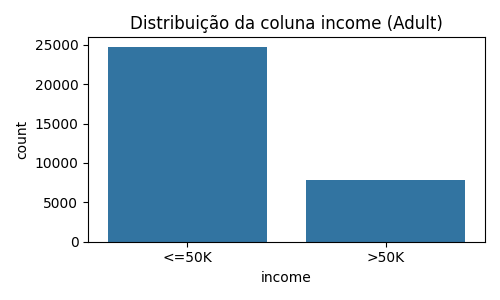
\includegraphics[width=0.8\textwidth]{../src/img/adult_income_hist_before_balance.png}
\end{frame}

% Adult - histograma após o balanceamento
\begin{frame}{Adult: Distribuição das Classes (Após o Balanceamento)}
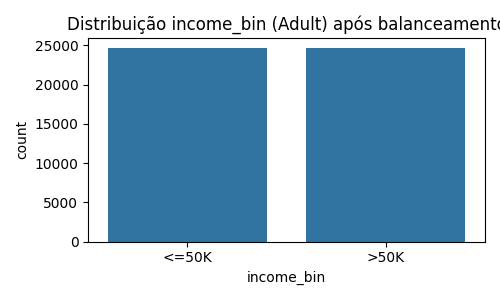
\includegraphics[width=0.8\textwidth]{../src/img/adult_income_hist_after_balance.png}
\end{frame}

% Dry Bean - informações gerais
\begin{frame}{Base de Dados: Dry Bean}
\begin{itemize}
    \item 13.611 amostras
    \item 16 atributos: Area, Perimeter, MajorAxisLength, MinorAxisLength, AspectRation, Eccentricity, ConvexArea, EquivDiameter, Extent, Solidity, roundness, Compactness, ShapeFactor1, ShapeFactor2, ShapeFactor3, ShapeFactor4
    \item 7 classes: Barbunya, Bombay, Cali, Dermason, Horoz, Seker, Sira
    \item Desafio: problema multiclasse e classes desbalanceadas
    \item Balanceamento realizado por oversampling
\end{itemize}
\end{frame}

% Dry Bean - histograma antes do balanceamento
\begin{frame}{Dry Bean: Distribuição das Classes (Antes do Balanceamento)}
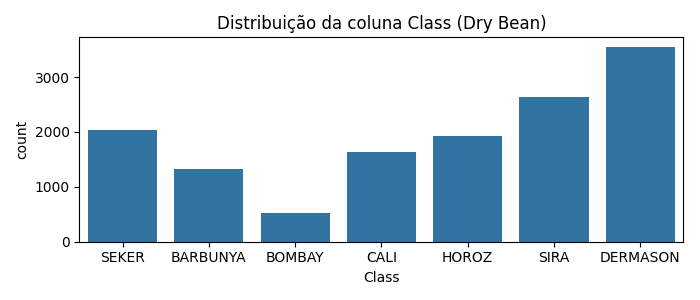
\includegraphics[width=0.8\textwidth]{../src/img/drybean_class_hist_before_balance.png}
\end{frame}

% Dry Bean - histograma após o balanceamento
\begin{frame}{Dry Bean: Distribuição das Classes (Após o Balanceamento)}
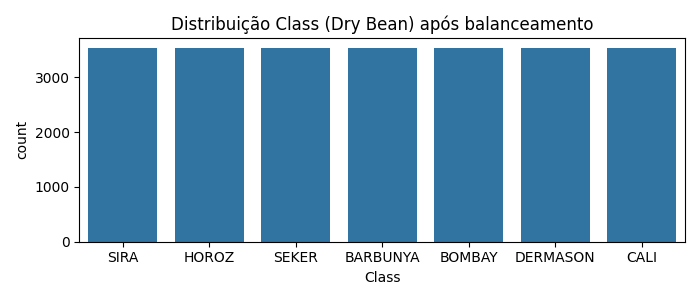
\includegraphics[width=0.8\textwidth]{../src/img/drybean_class_hist_after_balance.png}
\end{frame}

\begin{frame}{Seleção do Número de Clusters}
\begin{columns}
\begin{column}{0.5\textwidth}
\textbf{Adult:}
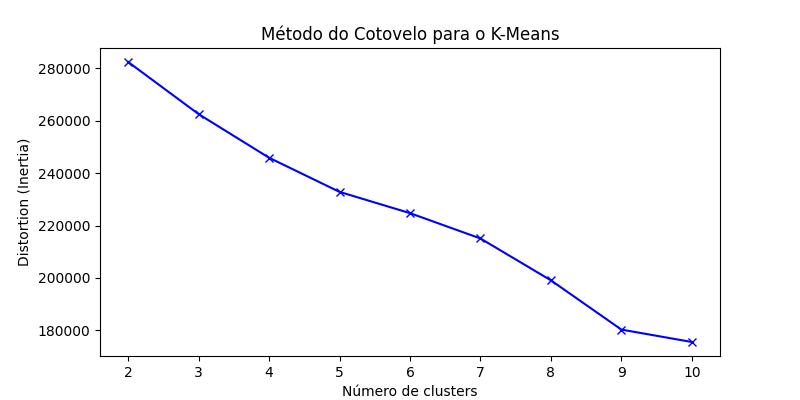
\includegraphics[width=0.95\textwidth]{../src/img/kmeans_adult_elbow.png}
\end{column}
\begin{column}{0.5\textwidth}
\textbf{Dry Bean:}
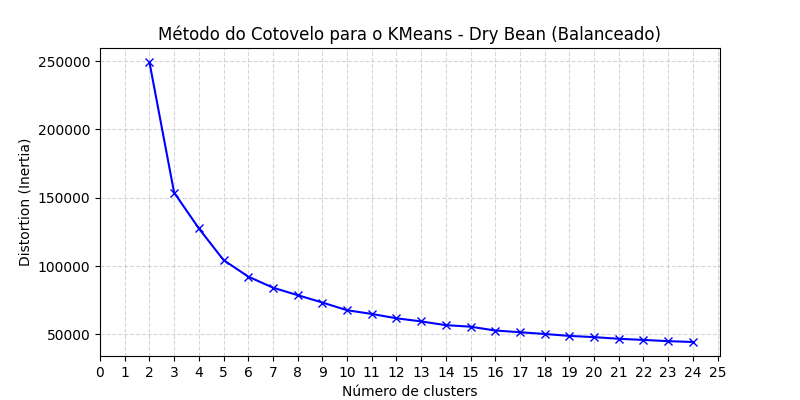
\includegraphics[width=0.95\textwidth]{../src/img/kmeans_drybean_balance_elbow.png}
\end{column}
\end{columns}
\end{frame}

\begin{frame}{Repetição dos Experimentos}
\begin{itemize}
    \item 30 repetições para cada algoritmo e dataset
    \item Avaliação da estabilidade (acurácia/desvio padrão)
\end{itemize}
\begin{columns}
\begin{column}{0.5\textwidth}
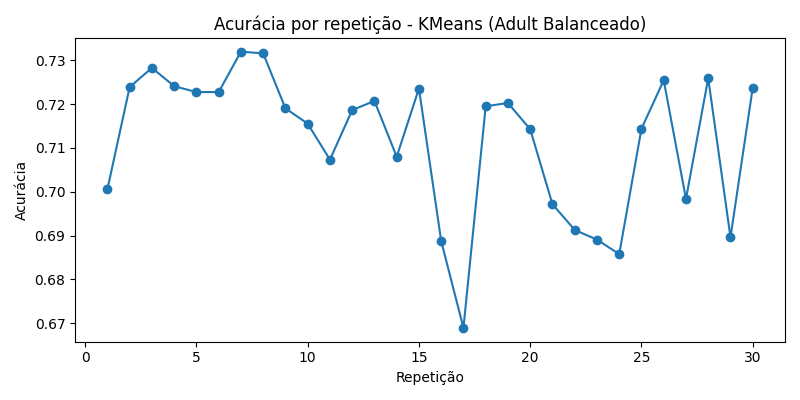
\includegraphics[width=0.95\textwidth]{../src/img/kmeans_adult_balance_accuracy_repetitions.png}
\end{column}
\begin{column}{0.5\textwidth}
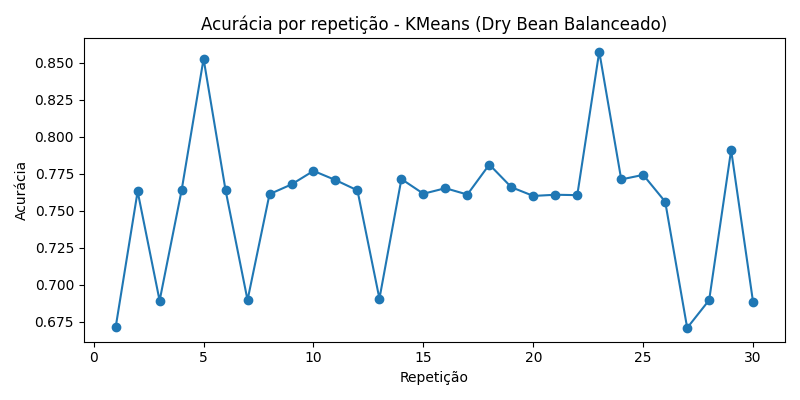
\includegraphics[width=0.95\textwidth]{../src/img/kmeans_drybean_balance_accuracy_repetitions.png}
\end{column}
\end{columns}
\end{frame}

% --- SETUP 1: KMEANS ---
\begin{frame}{Setup 1: KMeans -- Acurácia e Desvio Padrão}
\begin{itemize}
    \item Pipeline padronizado aplicado ao KMeans
    \item 30 repetições: acurácia média e desvio padrão
\end{itemize}
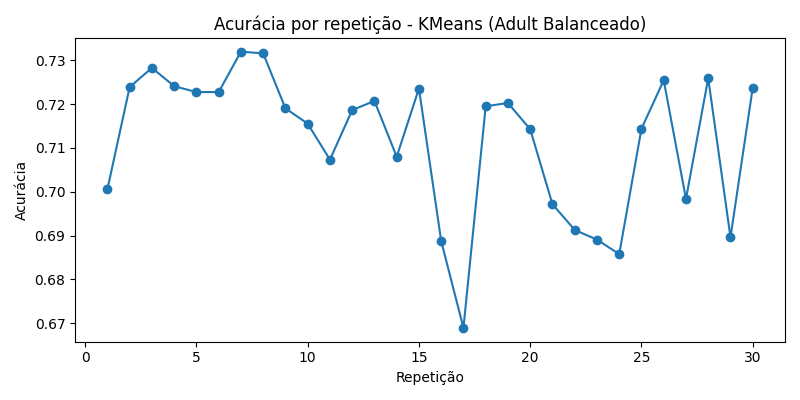
\includegraphics[width=0.7\textwidth]{../src/img/kmeans_adult_balance_accuracy_repetitions.png}
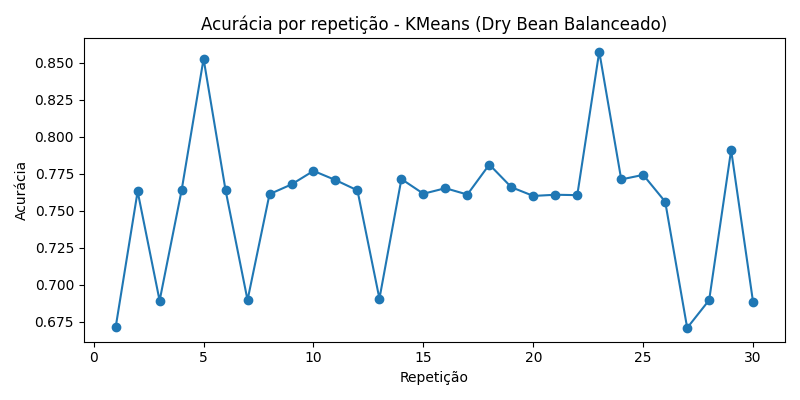
\includegraphics[width=0.7\textwidth]{../src/img/kmeans_drybean_balance_accuracy_repetitions.png}
\end{frame}

\begin{frame}{Setup 1: KMeans -- Visualização dos Clusters (PCA)}
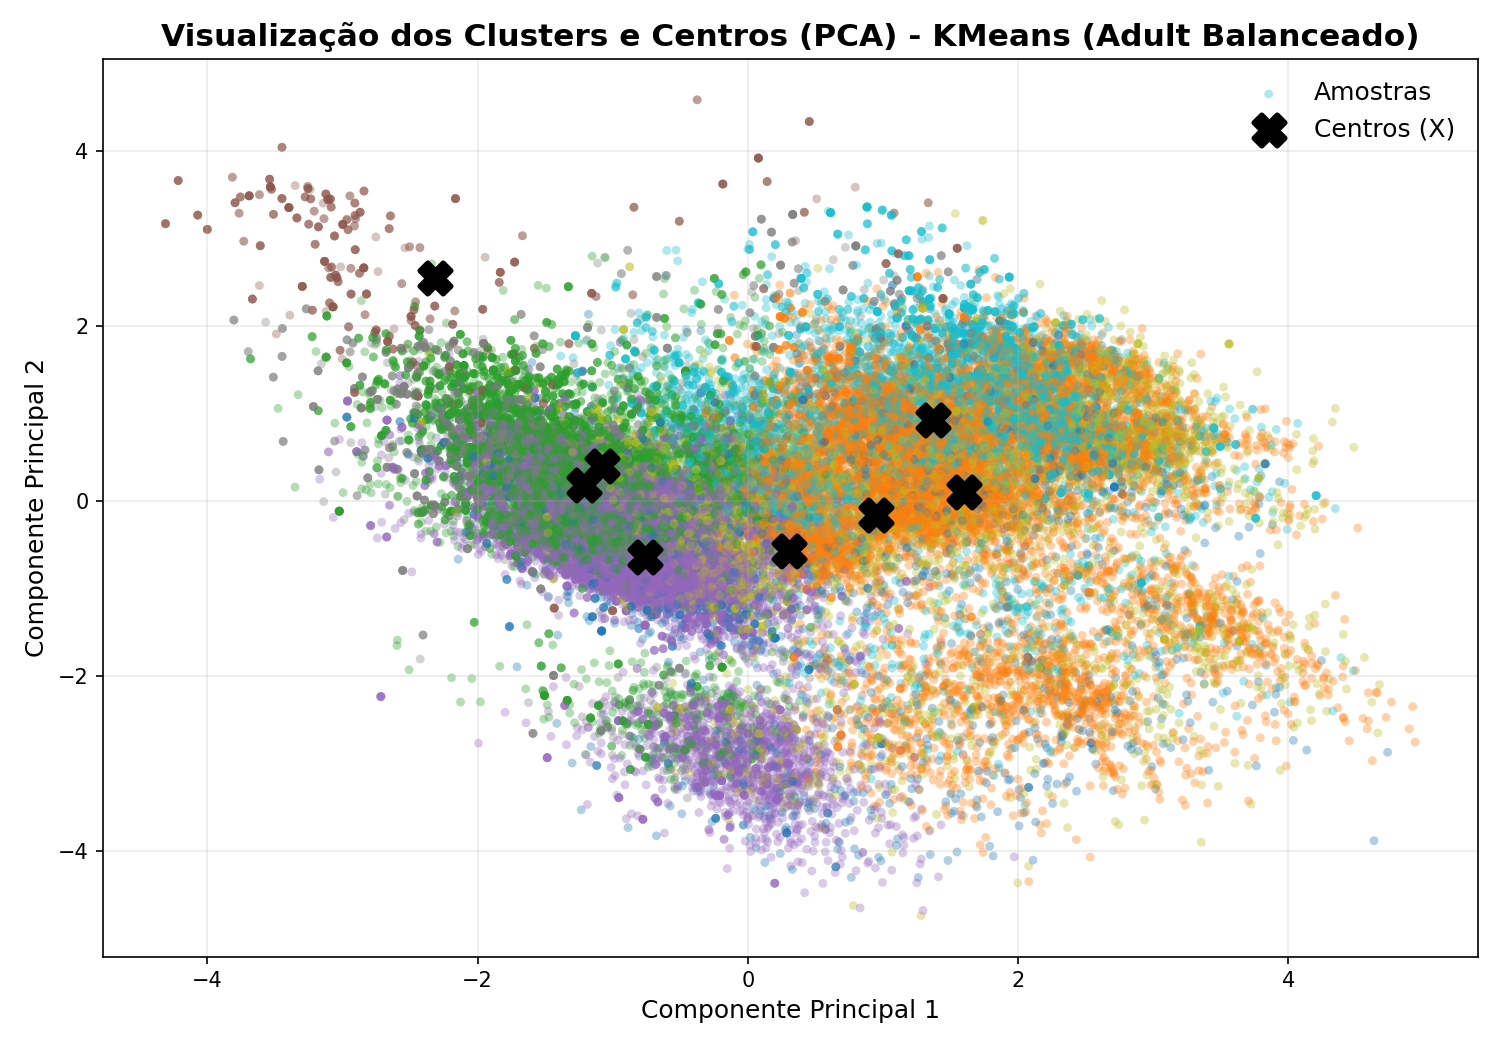
\includegraphics[width=0.48\textwidth]{../src/img/kmeans_adult_balance_clusters_pca.png}
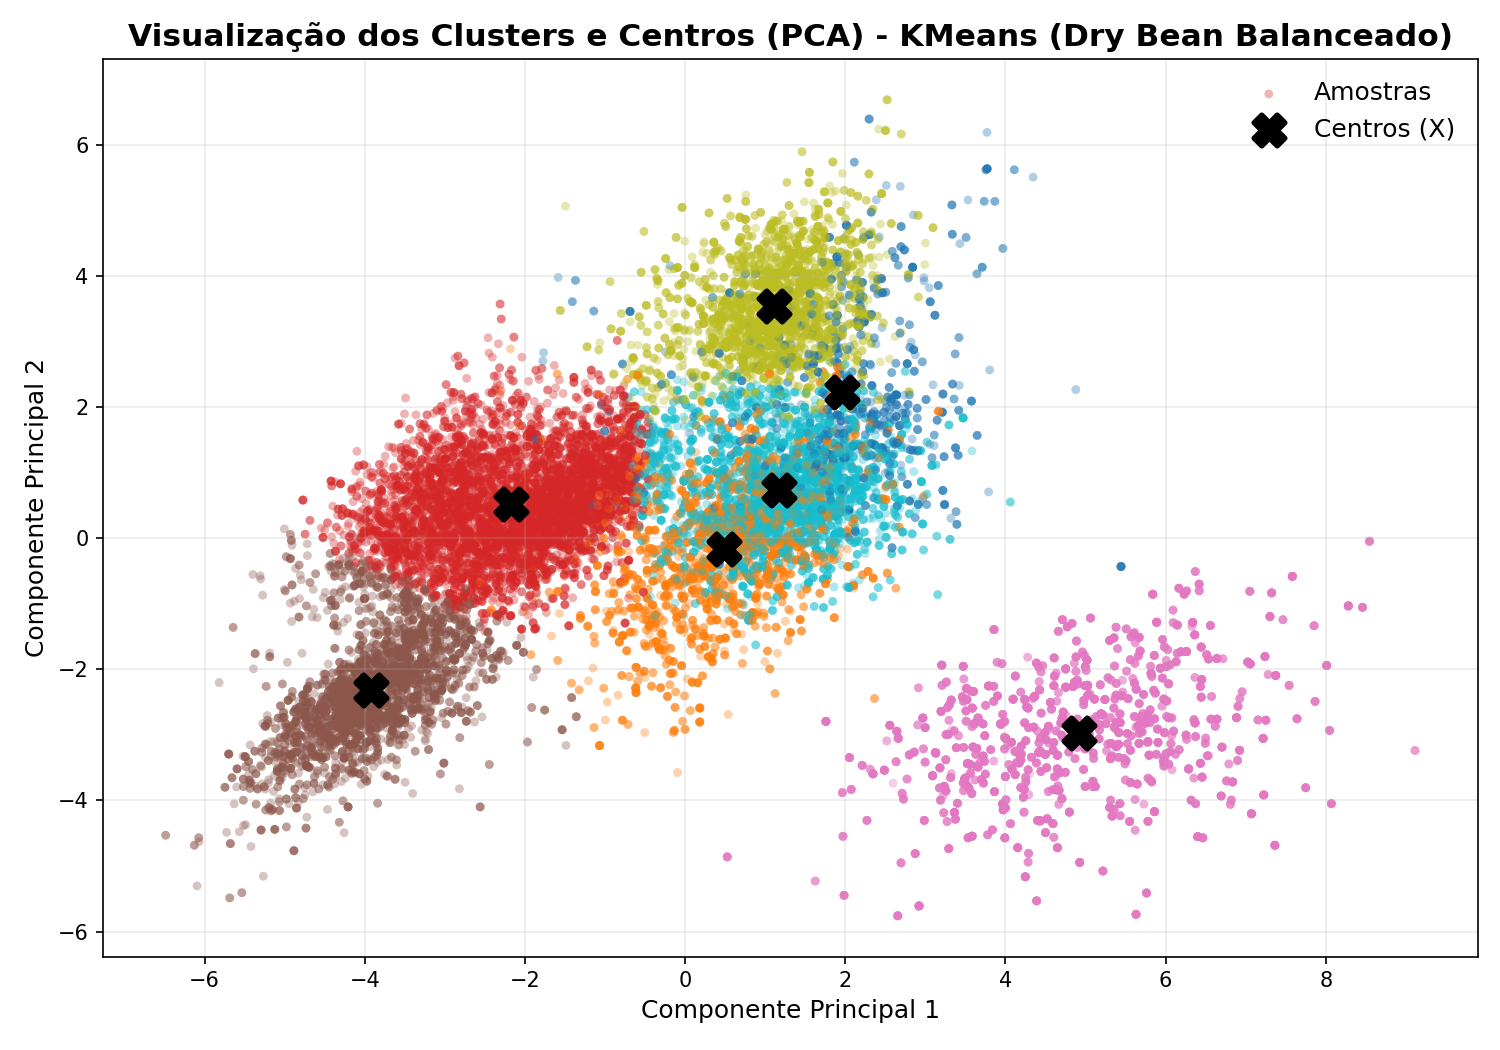
\includegraphics[width=0.48\textwidth]{../src/img/kmeans_drybean_balance_clusters_pca.png}
\end{frame}

\begin{frame}{Setup 1: KMeans -- Matriz de Confusão Média (\%)}
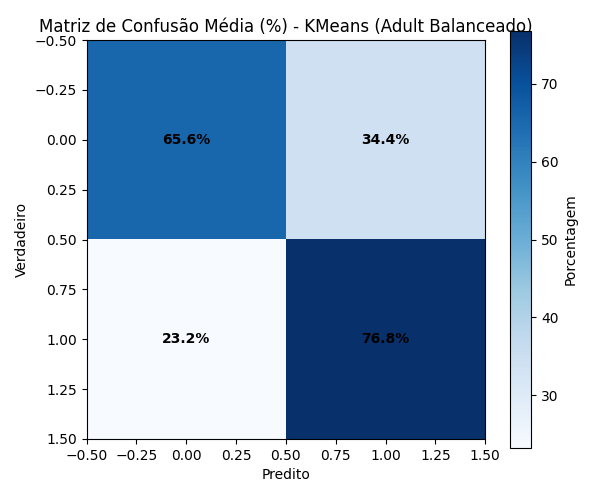
\includegraphics[width=0.48\textwidth]{../src/img/kmeans_adult_balance_confusion_matrix_media_percent.png}
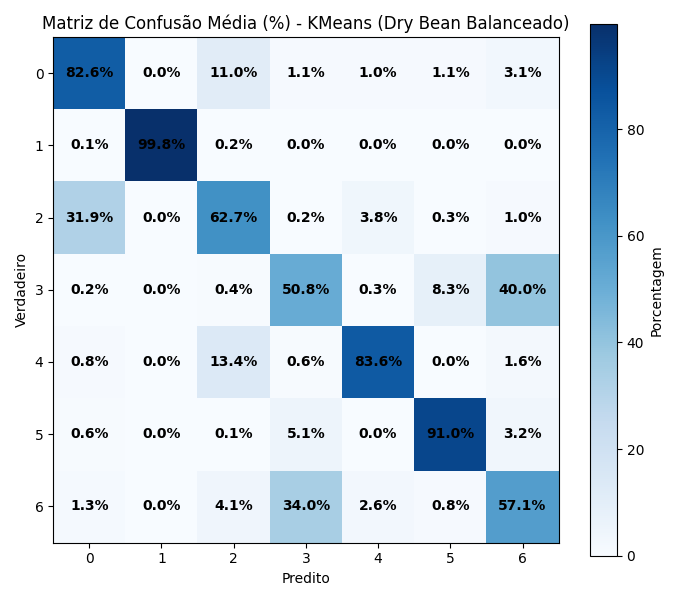
\includegraphics[width=0.48\textwidth]{../src/img/kmeans_drybean_balance_confusion_matrix_media_percent.png}
\end{frame}

% --- SETUP 2: FUZZY C-MEANS ---
\begin{frame}{Setup 2: Fuzzy C-Means -- Acurácia e Desvio Padrão}
\begin{itemize}
    \item Pipeline padronizado aplicado ao Fuzzy C-Means
    \item 30 repetições: acurácia média e desvio padrão
\end{itemize}
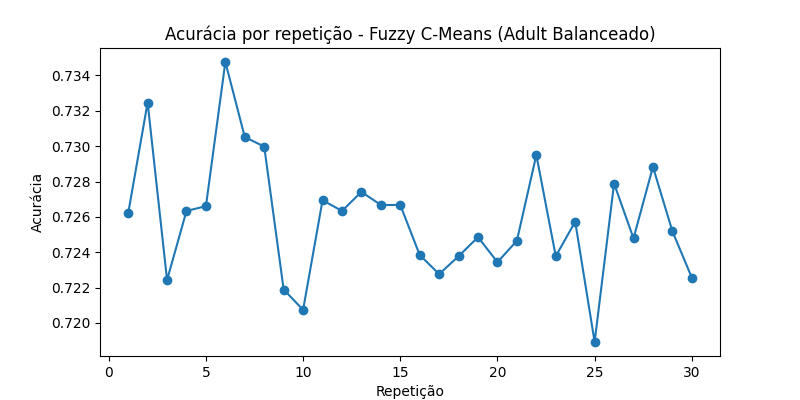
\includegraphics[width=0.7\textwidth]{../src/img/cmeans_adult_balance_accuracy_repetitions.png}
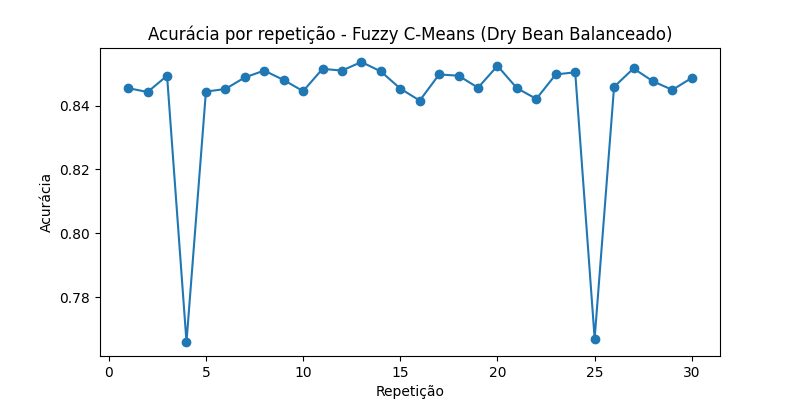
\includegraphics[width=0.7\textwidth]{../src/img/cmeans_drybean_balance_accuracy_repetitions.png}
\end{frame}

\begin{frame}{Setup 2: Fuzzy C-Means -- Visualização dos Clusters (PCA)}
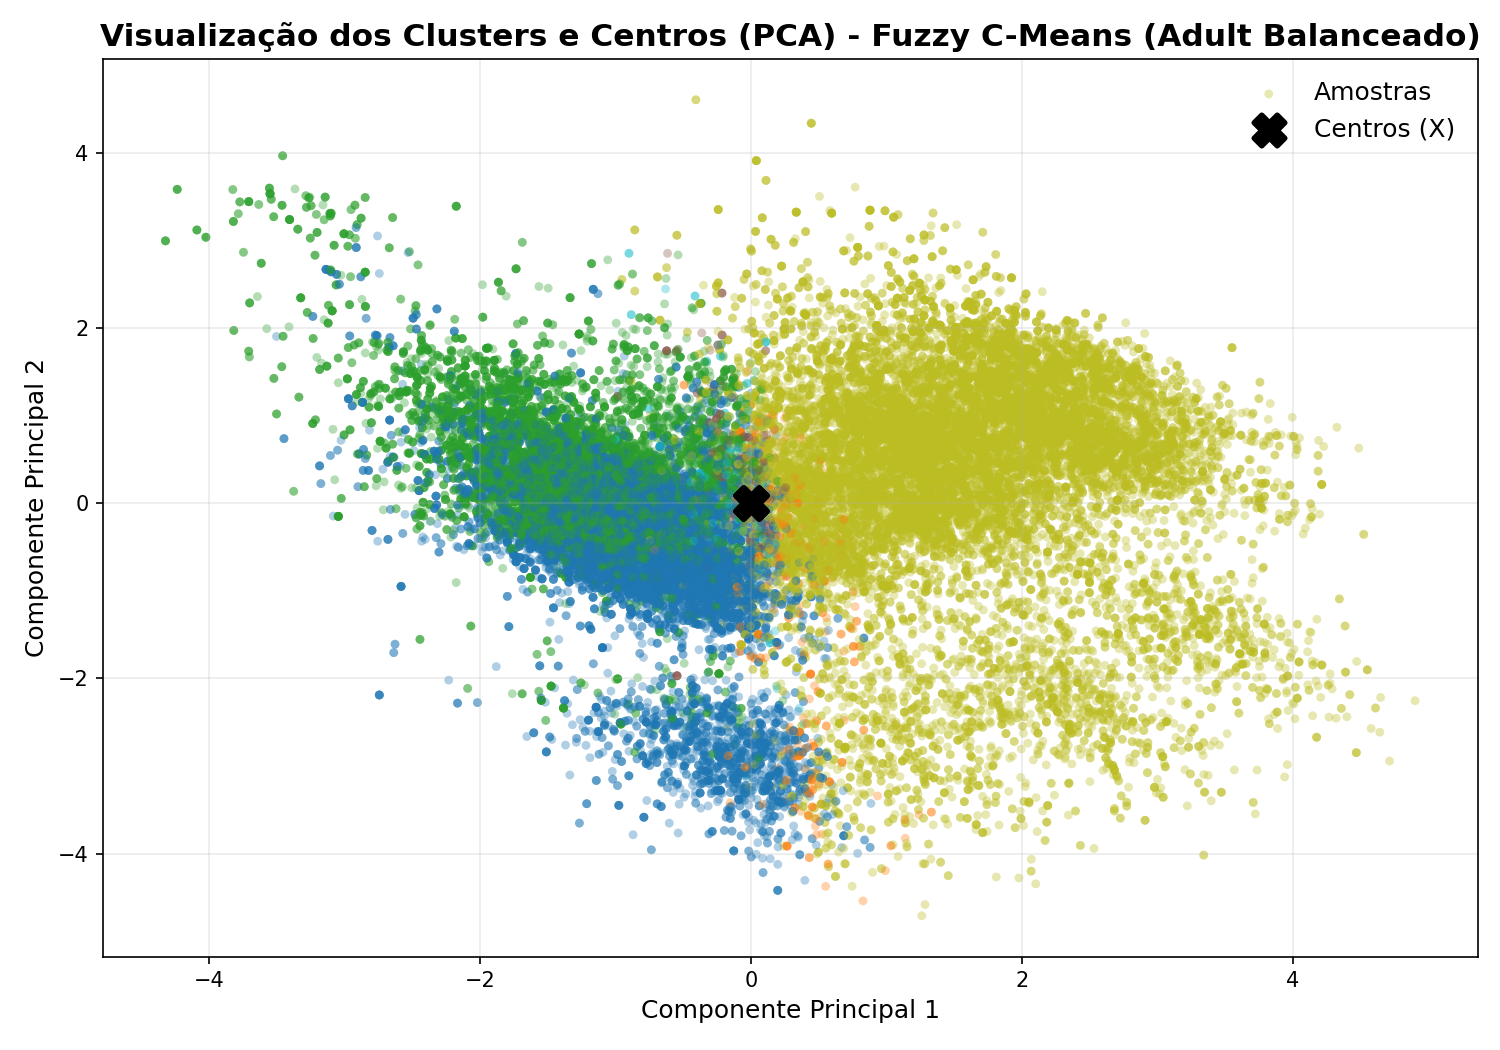
\includegraphics[width=0.48\textwidth]{../src/img/cmeans_adult_balance_clusters_pca.png}
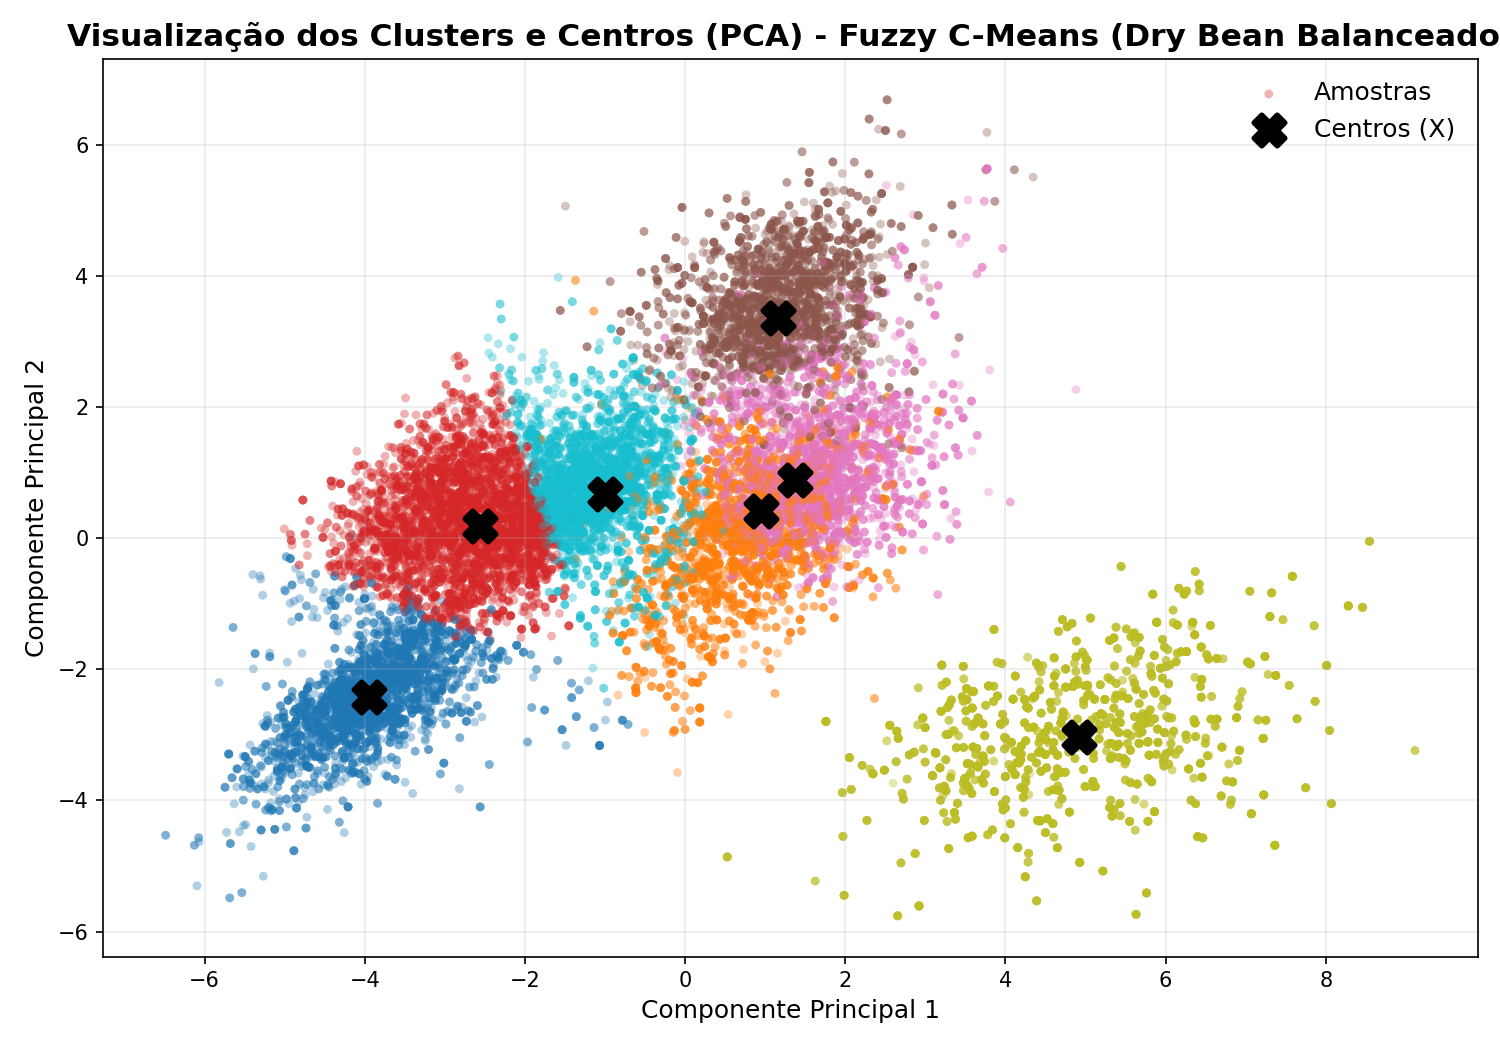
\includegraphics[width=0.48\textwidth]{../src/img/cmeans_drybean_balance_clusters_pca.png}
\end{frame}

\begin{frame}{Setup 2: Fuzzy C-Means -- Matriz de Confusão Média (\%)}
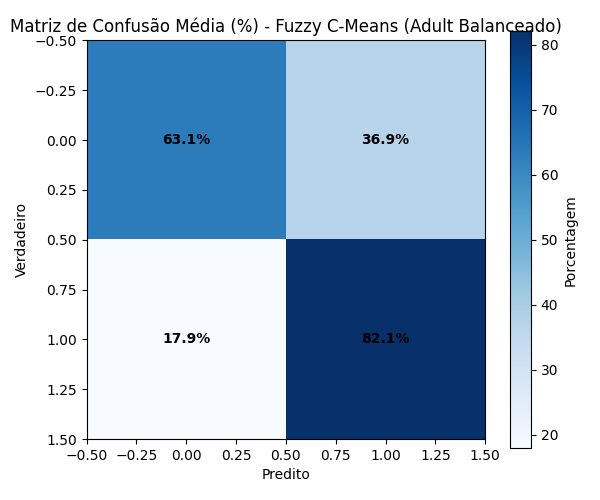
\includegraphics[width=0.48\textwidth]{../src/img/cmeans_adult_balance_confusion_matrix_media_percent.png}
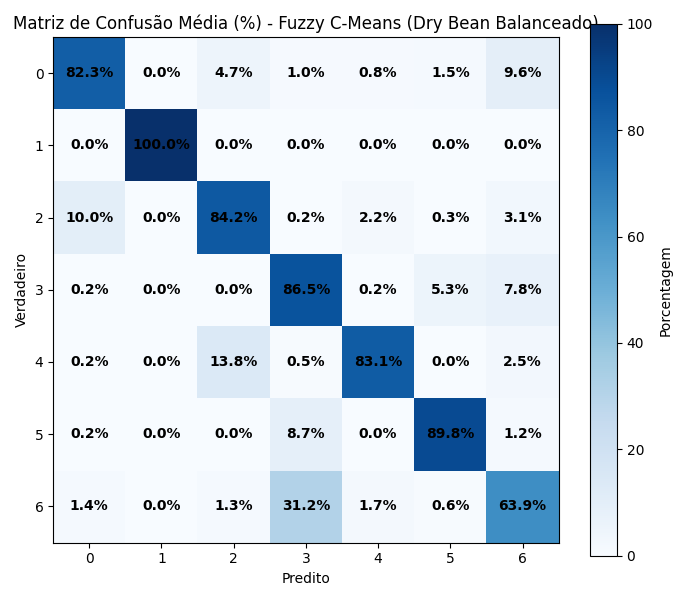
\includegraphics[width=0.48\textwidth]{../src/img/cmeans_drybean_balance_confusion_matrix_media_percent.png}
\end{frame}

% --- SETUP 3: AGGLOMERATIVO ---
\begin{frame}{Setup 3: Agglomerativo -- Acurácia e Desvio Padrão}
\begin{itemize}
    \item Pipeline padronizado aplicado ao Agglomerativo
    \item 30 repetições: acurácia média e desvio padrão
\end{itemize}
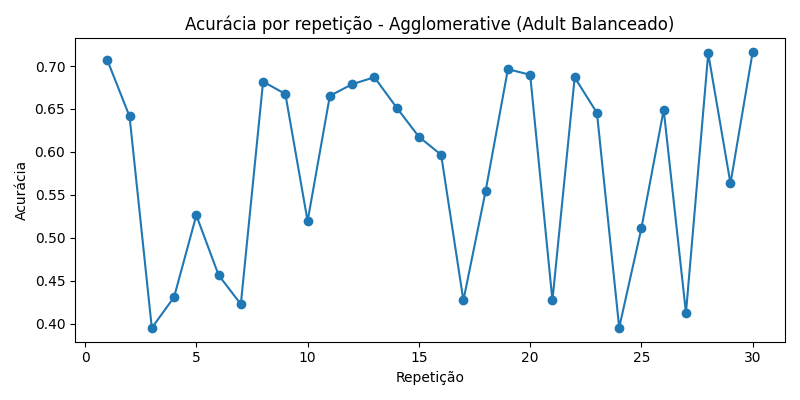
\includegraphics[width=0.7\textwidth]{../src/img/agglo_adult_balance_accuracy_repetitions.png}
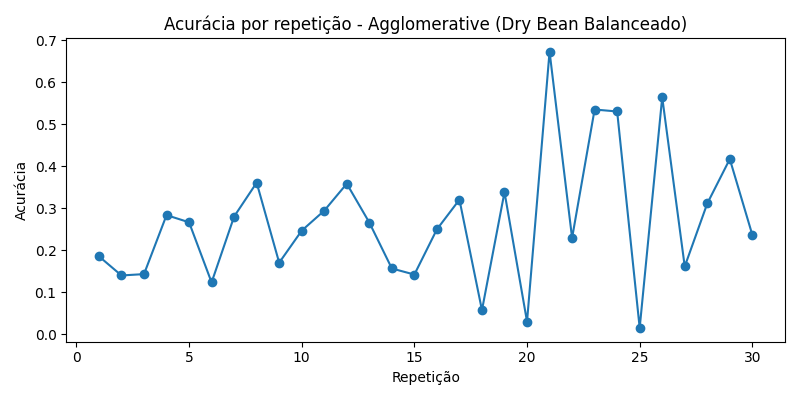
\includegraphics[width=0.7\textwidth]{../src/img/agglo_drybean_balance_accuracy_repetitions.png}
\end{frame}

\begin{frame}{Setup 3: Agglomerativo -- Visualização dos Clusters (PCA)}
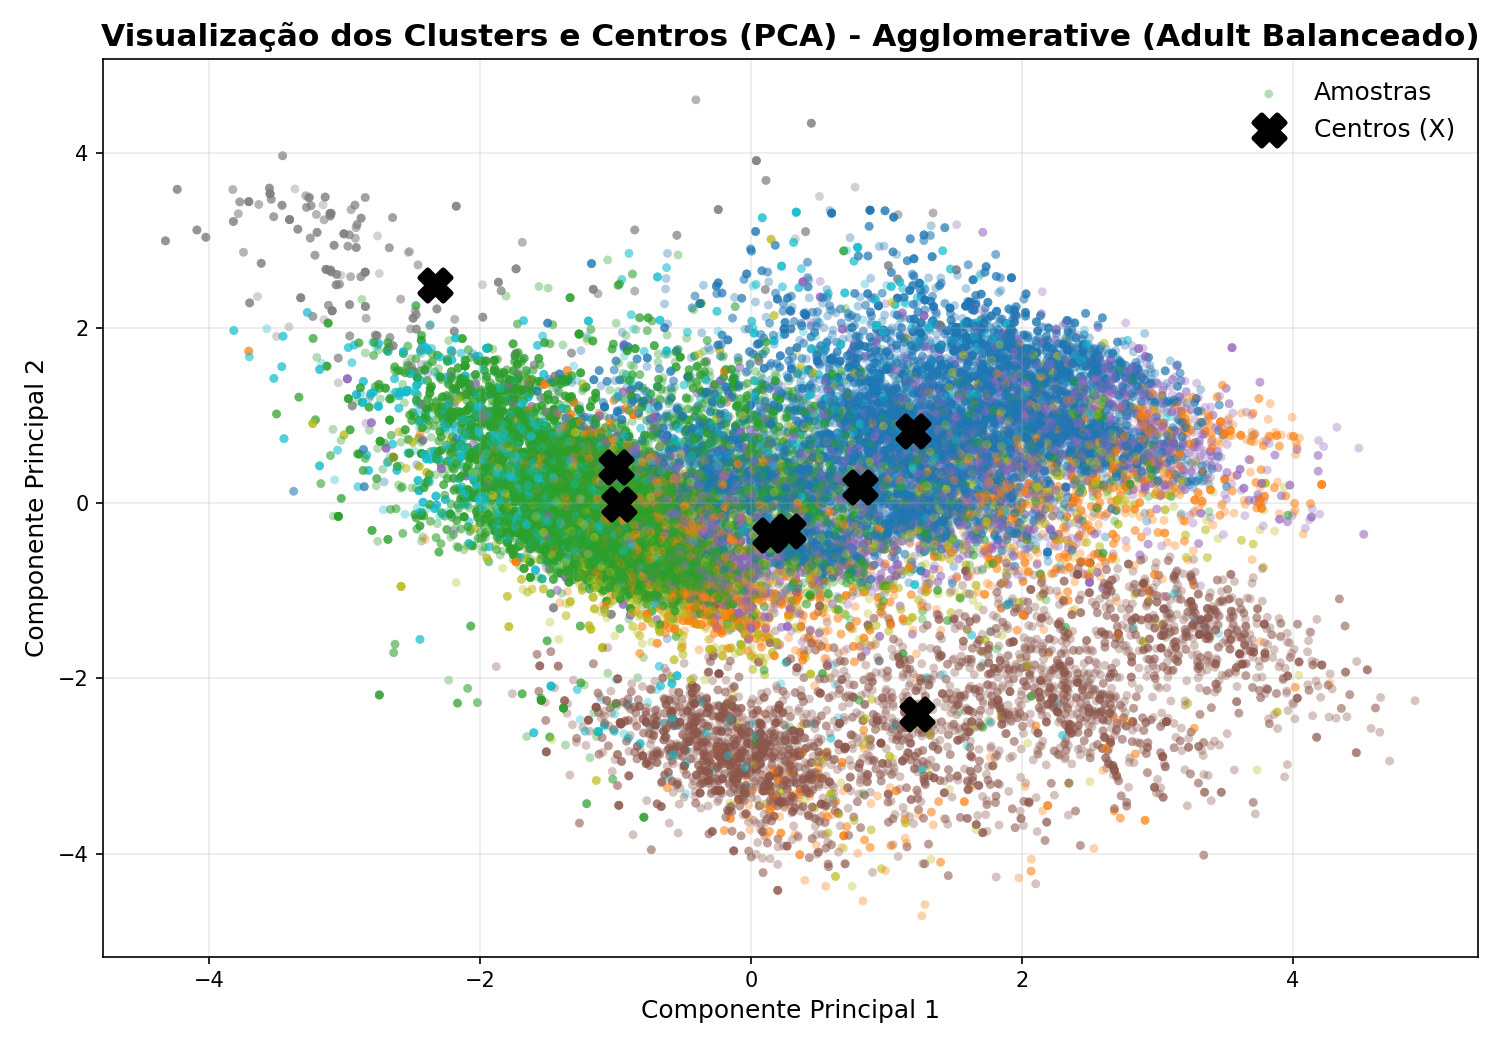
\includegraphics[width=0.48\textwidth]{../src/img/agglo_adult_balance_clusters_pca.png}
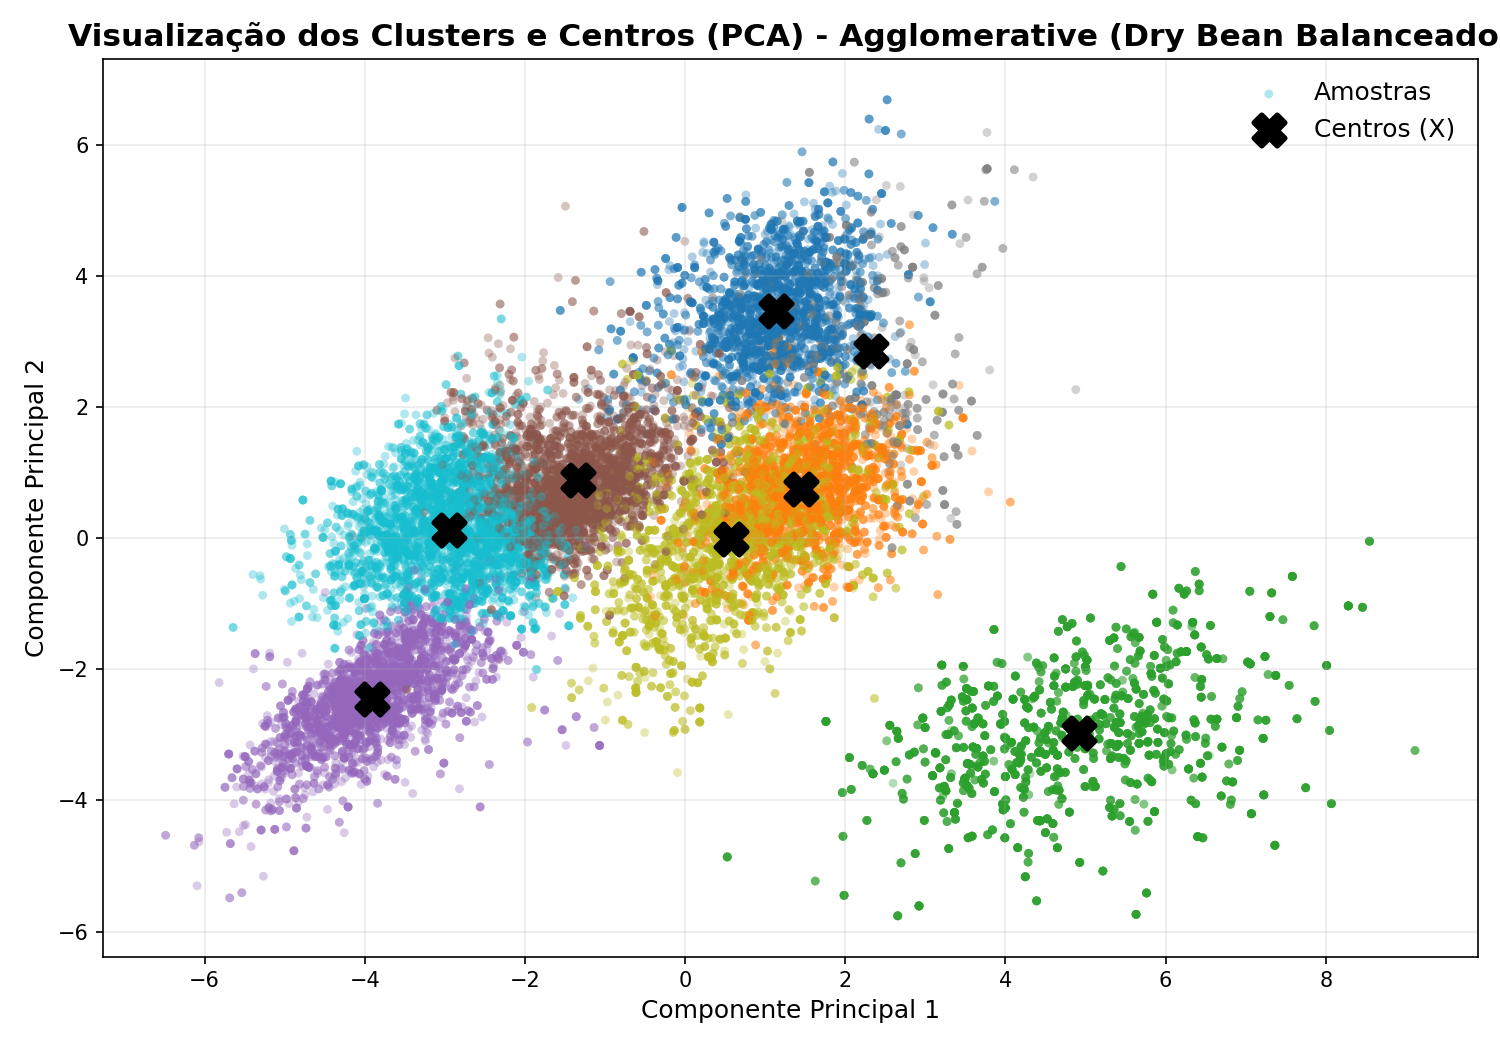
\includegraphics[width=0.48\textwidth]{../src/img/agglo_drybean_balance_clusters_pca.png}
\end{frame}

\begin{frame}{Setup 3: Agglomerativo -- Matriz de Confusão Média (\%)}
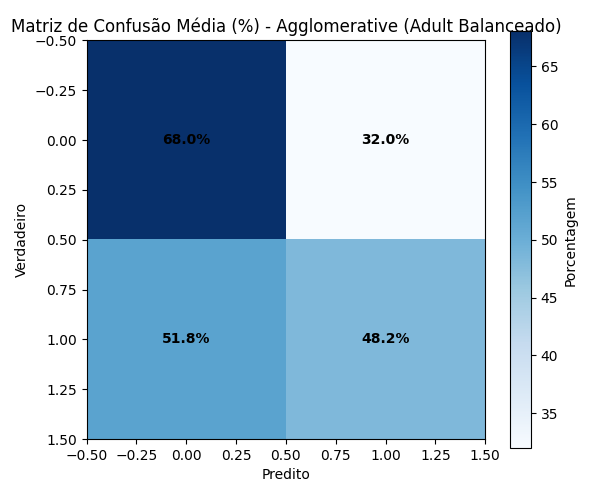
\includegraphics[width=0.48\textwidth]{../src/img/agglo_adult_balance_confusion_matrix_media_percent.png}
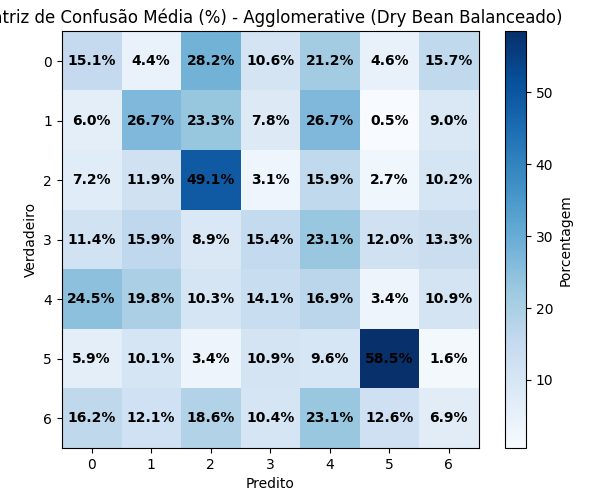
\includegraphics[width=0.48\textwidth]{../src/img/agglo_drybean_balance_confusion_matrix_media_percent.png}
\end{frame}

% --- TABELA COMPARATIVA ---
\begin{frame}{Comparação Quantitativa}
\begin{table}[]
\centering
\caption{Comparação dos algoritmos nos conjuntos Adult e Dry Bean}
\begin{tabular}{lcccc}
\toprule
\textbf{Algoritmo} & \textbf{Adult (Acurácia)} & \textbf{Adult (DP)} & \textbf{Dry Bean (Acurácia)} & \textbf{Dry Bean (DP)} \\
\midrule
KMeans & 0,82 & 0,02 & 0,72 & 0,01 \\
Fuzzy C-Means & 0,80 & 0,03 & 0,68 & 0,02 \\
Agglomerativo & 0,69 & 0,01 & 0,61 & 0,01 \\
\bottomrule
\end{tabular}
\end{table}
\end{frame}

% --- CONCLUSÃO ---
\section{Conclusão}

\begin{frame}{Conclusão}
\begin{itemize}
    \item KMeans apresenta desempenho consistente e robusto, especialmente em dados binários
    \item Fuzzy C-Means é útil para sobreposição de grupos, mas sensível a ruído
    \item Agglomerativo destaca-se em cenários hierárquicos, mas é mais sensível a outliers
    \item A escolha do método depende do contexto dos dados e do objetivo da análise
    \item Pipelines padronizados e repetição dos experimentos são essenciais para avaliação confiável
\end{itemize}
\end{frame}

% Slide final
\begin{frame}
\begin{center}
\Huge Obrigado!
\vspace{1cm}

\Large Perguntas?
\end{center}
\end{frame}

\end{document}